\documentclass{vldb}

\usepackage{latexsym}
\usepackage{amsmath}
\usepackage{algorithmic}
\usepackage{algorithm}
\usepackage{clrscode}
%\usepackage{epsfig}
%\usepackage{epic}
%\usepackage{eepic}
%\usepackage{xspace}
\usepackage{pst-tree}

%\addtolength{\textwidth}{1in}
%\addtolength{\oddsidemargin}{-0.5in}
%\addtolength{\evensidemargin}{-0.5in}
%\addtolength{\textheight}{0.8in}
%\addtolength{\topmargin}{-0.5in}
%\leftmargini 2.9ex


\def\punto{$\hspace*{\fill}\Box$}
\newcommand{\nop}[1]{}
\newcommand{\tuple}[1]{{\langle#1\rangle}}
\def\lBrack{\lbrack\!\lbrack}
\def\rBrack{\rbrack\!\rbrack}
\newcommand{\Bracks}[1]{\lBrack#1\rBrack}


\newtheorem{theorem}{Theorem}[section]
\newtheorem{metatheorem}{Metatheorem}[section]
\newtheorem{example}[theorem]{Example}
%\newtheorem{algorithm}[theorem]{Algorithm}
\newtheorem{definition}[theorem]{Definition}
\newtheorem{proposition}[theorem]{Proposition}
\newtheorem{property}[theorem]{Property}
\newtheorem{corollary}[theorem]{Corollary}
\newtheorem{lemma}[theorem]{Lemma}
\newtheorem{remark}[theorem]{Remark}
\newtheorem{conjecture}[theorem]{Conjecture}
\newtheorem{proviso}[theorem]{Proviso}
\newtheorem{todo}[theorem]{ToDo}

\newcommand{\comment}[1]{}
\newcommand{\compiler}{DBToaster}
\newcommand{\project}{Steam}

\title{DBToaster: Compiling main-memory database query~processors}

\numberofauthors{1}

\author{
\alignauthor Yanif Ahmad and Christoph Koch \\
\affaddr{Department of Computer Science} \\
\affaddr{Cornell University, Ithaca, NY} \\
\email{\{yanif, koch\}@cs.cornell.edu}}
\date{}


\toappear{}


\begin{document}


\maketitle


\begin{abstract}
We  present a novel  SQL query  compilation framework  which generates native 
code that incrementally  and continuously  maintains aggregate views  in main 
memory at  high  update rates  using delta  processing techniques. DBToaster, 
our compiler, generates C++  code that  performs all the  processing required 
for an input  tuple as  a simple  straight-line function. Thus we turn  a fixed,
optimized query plan into code that can be further optimized by a C++ compiler,
and avoid overheads that traditionally arise when query processors interpret
query plans stored in dynamic data structures. Our new delta processing
techniques are designed specifically for compilation to native code and support
aggressive inlining that leads to surprisingly small and simple straight-line
code sequences.

Our  work  is  motivated  by  applications  that  require  the  highly
efficient answering of fixed workloads of aggregation queries, such as
in  data stream  processing,  online data  warehouse  loading, and  in
financial applications. As we  show, our techniques are several orders
of  magnitude   faster  than  state-of-the-art   database  and  stream
processing engines on such workloads.  In the case of queries on limit
order  book  data  as  required for  supporting  algorithmic  equities
trading, our approach currently stands alone in its ability to support
realistic  data rates  on contemporary  hardware without  resorting to
very substantial computing clusters.
\end{abstract}



In recent years, algorithmic trading systems have come to account for a majority
of volume traded at the major US and European financial markets (for instance,
for 73\% of all US equity trading volume in the first quarter of 2009
\cite{Iati2009}). The success of automated trading systems depends critically on
strategy processing speeds: trading systems that react faster to market events
tend to make money at the cost of slower systems. Unsurprisingly, algorithmic
trading has become a substantial source of business for the IT industry; for
instance, it is the leading vertical among the customer bases for high-speed
switch manufacturers (e.g., Arista \cite{Becht2010}) and data stream processing.




A typical algorithmic trading system is run by mathematicians who develop
trading strategies and by programmers and systems experts who implement these
strategies to perform fast enough, using mainly low-level programming languages
such as C. Developing trading strategies requires a feedback loop of simulation,
back-testing with historical data, and strategy refinement based on the insights
gained. This loop, and the considerable amount of low-level programming that it
causes, is the root of a very costly {\em productivity bottleneck}\/: in fact,
the number of programmers often exceeds the number of strategy designers by
an order of magnitude.


Trading algorithms often perform a considerable amount of data crunching
and statistical processing that could in principle be implemented using SQL
views, coupled with some relatively straightforward control and trading logic.
%
Differently from other areas of finance such as technical analysis,
where stream processing engines
\cite{abadi-vldbj:03,motwani-cidr:03} can be applied,
data processing in trading algorithms using views cannot be performed by DBMS or
data stream processing systems today: the former are not able to (1) {\em update
their views at the required rates}\/ (for popular stocks, hundreds of orders per
second may be executed, even outside burst times) and the latter are not able to
(2) {\em maintain large enough data state}\/ and support suitable query
languages (non-windowed SQL aggregates) on this state.

%
A data management system that could handle these two requirements would yield a
very substantial productivity increase that can be directly monetized -- the
holy grail of algorithmic trading.

Trading algorithms often perform a considerable amount of data crunching that
could in principle be implemented as SQL views, but cannot be achieved by DBMS
or data stream processing systems today: DBMS are not able to (1) {\em update
their views at the required rates}\/ (for popular stocks, hundreds of orders per
second may be executed, even outside burst times) and stream engines are not
able to (2) {\em maintain large enough data state}\/ and support suitable query
languages (non-windowed SQL aggregates) on this state.
A data management system fulfilling these two requirements would yield a very
substantial productivity increase that can be directly monetized -- the holy
grail of algorithmic trading.



To understand the need to maintain and query a large data state, note that
many stock exchanges provide a detailed view of the market microstructure
through complete bid and ask {\em limit order books}. The bid order book is a
table of purchase offers with their prices and volumes, and correspondingly the
ask order book indicates investors' selling orders. Exchanges execute trades by
matching bids and asks by price and favoring earlier timestamps. Investors
continually add, modify or withdraw limit orders, thus one may view order books
as relational tables subject to high update volumes. The availability of order
book data has provided substantial opportunities for automatic algorithmic
trading.





To illustrate this, we describe the Static Order Book Imbalance (SOBI) trading
strategy. SOBI computes a volume-weighted average price (VWAP) over those orders
whose volume makes up a fixed upper $k$-fraction of the total stock volume in
both bid and ask order books. SOBI then compares the two VWAPs and, based on
this, predicts a future price drift (for example a bid VWAP larger than an ask
VWAP indicates demand exceeds supply, and prices may rise). For simplicity, we
present the VWAP for the bids only:



\begin{verbatim}
select avg(b2.price * b2.volume) as bid_vwap
from   bids b2
where  k * (select sum(volume) from bids)
         > (select sum(volume) from bids b1
            where b1.price > b2.price);
\end{verbatim}
\comment{
Focusing on the $k$-fraction of the order book closest to the current price
makes the SOBI strategy less prone to attacks known as {\em axes}\/ (large
tactical orders far from the current price that will thus not be executed but
may confuse competing algorithms).
}


Coming back to our two desiderata, for trading algorithms to be successful, (1)
views such as VWAP need to be maintained and monitored by the algorithms at or
close to the trading rate. However, (2) the views cannot be expressed through
time-, row- or punctuation-based window semantics.




\begin{figure}
\begin{center}
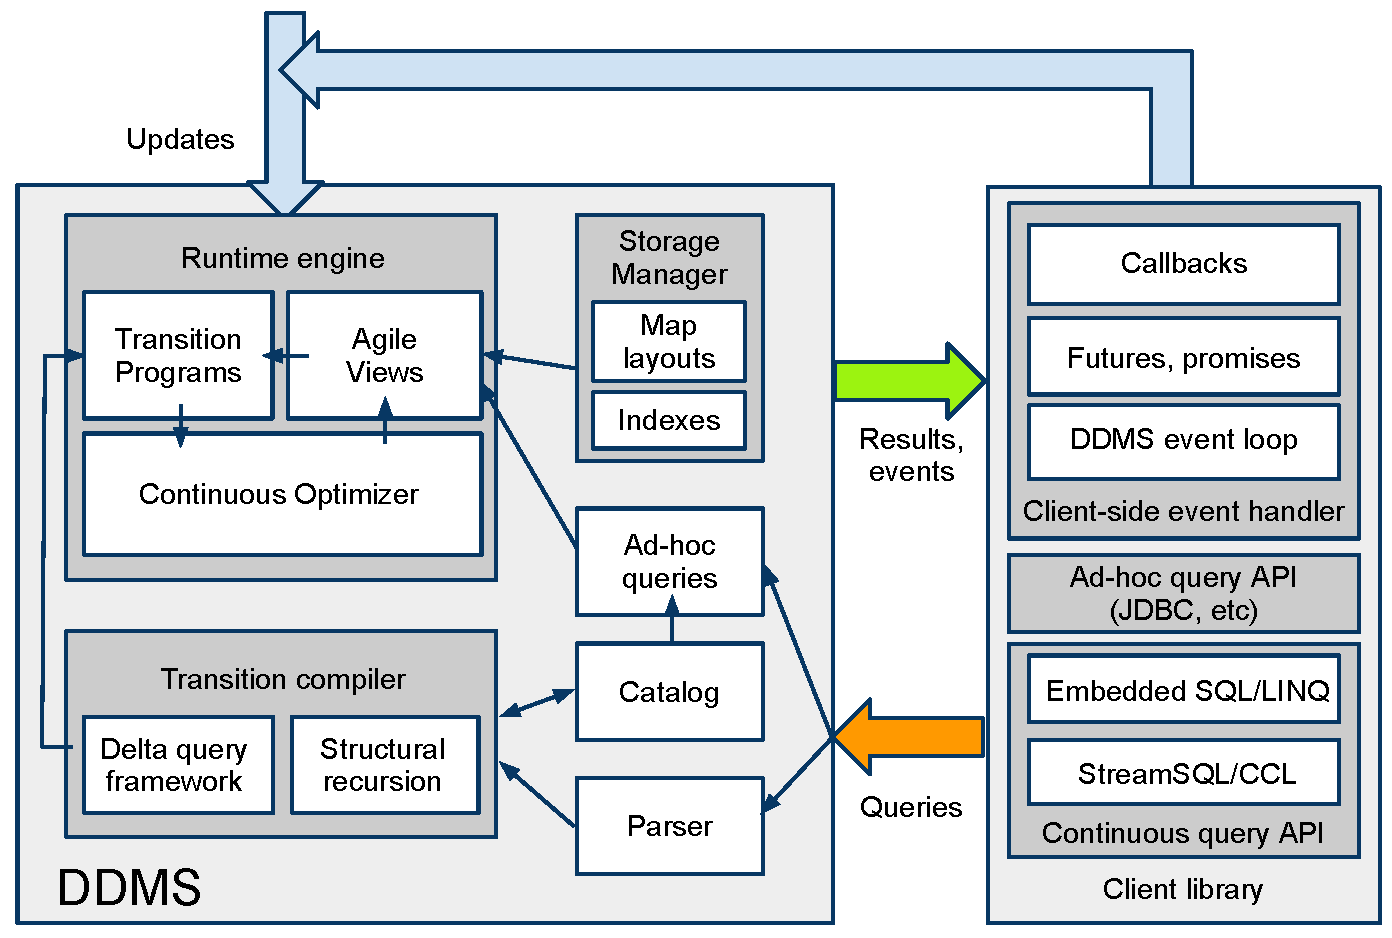
\includegraphics[width=3.3in]{graphics/CIDRarch.pdf}
\end{center}
\vspace*{-0.2in}
\caption{Dynamic Data Management System (DDMS) and Application Interface
Architecture}
\label{fig:ddmsarch}
\vspace*{-0.2in}
\end{figure}

We now examine the architecture of a DDMS, as illustrated in Figure
\ref{fig:ddmsarch}.  The core component of a DDMS is its runtime engine.  Unlike
a traditional database system where the same engine manages all database
instances, each individual DDMS execution runtime is constructed around a
specific set of queries provided by the client program (e.g., via SQL code
embedded inline in the program), each defining an \textit{agile view}.

\subsection{Application Interfaces}

The data that is processed by a DDMS arrives at the system in the form of an
update stream of tuple insertions, deletions and modifications. The stream need
not be ordered in any shape or form, and deletions are assumed to apply to
tuples that have already been seen at some arbitrary prior point on the stream.
Updates are fully processed on-the-fly, and their effects on agile views are
realised in atomic fashion, prior to working on any subsequent update. Depending
on the type of results requested by queries, any results arising from updates
will be directly forwarded to application code as agile views are maintained.

DBToaster provides a wide variety of client interfaces to issue queries and
obtain results from the DDMS, to reflect the diverse needs of applications built
on top of our tool. Today's stream processors tend to be black-box systems that
run completely decoupled from the application. Client libraries interact with
stream processors through remote procedure call abstractions, issuing queries
and new data through function calls, and either polling or being notified
whenever results appear on a queue that is associated with a TCP socket
connected to the stream processor.

In DBToaster, the set of agile views requested by clients, the \textit{visible
schema}, forms the primary read interface between client programs and the DDMS
runtime. Clients can submit queries for which the DDMS materializes an agile
view through three methods:
(1) a continuous query client API, as done with existing stream client
libraries, which sends a query string to the DDMS server for parsing,
compilation, and agile view construction. The query string may be specified in a
standard streaming language such as StreamSQL or CCL~\cite{jain-pvldb:08}. The
client may specify several ways to receive results, as seen below.
(2) an ad-hoc query client API, which issues a one-time query to the
DDMS, and returns the agile view as a datastructure to be used by the remainder
of the client program. This API may be used in both synchronous and
asynchronous modes, as indicated by the type of result requested. The query is
specified in standard SQL.
(3) an embedded language, whose syntax and data model are natural fits to the
host language in which the client application is written. Examples include
embedded SQL, and collection comprehension oriented approaches such as LINQ,
Links, and Ferry~\cite{meijer-sigmod:06,cooper-fmco:06,grust-sigmod:09}.
One interesting challenge with the embedded language approach is that of
enabling asynchronous event-driven programming. Whereas language embeddings
are natural for ad-hoc querying, we have yet to see these approaches
for stream processing.

Given these modes of issuing queries to the DDMS, our client interface supports
four methods of receiving results:
(1) callbacks, that can be specified as handlers as part of the continuous query
API. Callbacks receive a stream of query results, and are the simplest form of
result handlers that run to completion on query result events.  
(2) a DDMS event loop, which multiplexes result streams for multiple queries.
Applications may register callbacks to be executed on any result observed on the
event loop, allowing complex application behavior through dynamic
registration, observation and processing of results on the event loop.
(3) dynamic datastructures, which are read-only from the application
perspective. The datastructure appears as a native collection type in the host
language, facilitating natural access for the remainder of the program. Ad-hoc
queries use this method for results by default. Continuous queries may also use
this method in which case the datastructure acts as a proxy with accessors that
pull in any updates from the DDMS when invoked.
(4) promises and futures~\cite{Liskov:1988:PLS:53990.54016}, which provide a
push-based proxy datastructure for the
result. A future is an object whose value is not initially know and is provided
at a later time. A program using a query returning a future can use the future
as a native datatype, in essence constructing a client-side dataflow to be
executed whenever the future's value is bound. In our case, this occurs whenever
query results arrive from the DDMS. Language embedded stream processing can be
supported by futures, or program transformations to construct client side
dataflow, such as continuous passing style as found in the programming languages
literature~\cite{sussman-hsc:98}.


\comment{
An important distinction between the DDMS and a traditional DBMS is
that the DDMS treats both inputs (base relations in DBMS parlance) and agile views
(query outputs) as \textit{update streams} of tuple insertions, deletions and
revisions.  Updates are processed, and changes in the views are propagated
into the client.  If necessary, a DDMS runtime can also be instantiated with
support for ad-hoc queries.

The set of agile views requested by clients, the \textit{visible schema}, forms
the primary read interface between client programs and the DDMS runtime. This
interface comes in three flavors: (1) a push interface that invokes client
callbacks or schedules event handlers when a view in the visible schema changes,
(2) futures/promises representing queries over the visible schema that have not
yet been computed, or (3) read-only \textit{dynamic data structures}
representing each view in the visible schema.  One consequence of
limiting visibility into the database to the visible schema is that we are free
to represent a DDMS runtime's internal state in ways that are dramatically
different from a traditional DBMS.  We return to this observation later in the
paper.
}


\subsection{DDMS Internals}


%{\bf The runtime state machine}\/.
The internals of the runtime engine itself are best viewed through the lens of a
state machine.  Compared to similar abstractions for complex event
processors~\cite{agrawal-sigmod:08, demers-sigmod:07}, the state is
substantially larger. Conceptually, the state represents an entire
relational database and transitions represent changes in the base
relations: events in the update stream.



\tinysection{Compiling transitions}
Each transition causes maintenance work for our agile views, and just as
with incremental view maintenance, this work can be expressed as queries.
Maintenance can be aided by dynamic data structures, that is, additional agile
views making up the \textit{auxiliary schema}.
A DDMS is a long-running system, operating on a finite number of update streams.
This combination of characteristics naturally suggests \textit{compiling} and
specializing the runtime for each transition and associated maintenance
performed by a DDMS. The transition compiler generates lightweight transition
programs that can be invoked by the runtime engine with minimal overhead on the
arrival of events. We describe the compiler in further detail in Section
\ref{sec:dbtoaster}.




\tinysection{Storage management and ad-hoc query processing}
Given the instantiation of an auxiliary schema and agile views, a DDMS must
intelligently manage memory utilization, and memory-disk boundary as needed. The
storage manager of a DDMS is responsible for the efficient representation of
both the agile views, and any index structures required on these views.
Section~\ref{sec:storage} discusses the issue of indexing, as well as how views
are laid out onto disk. Supporting ad-hoc query processing turns out to be
relatively straightforward given the core of a DDMS continuously maintains agile
views. Ad-hoc queries can be rewritten to use agile views much in a similar
fashion to the materialized view usage problem in standard query optimization. A
key challenge here is how to ensure consistency, such that ad-hoc queries do not
use inconsistent agile views as update stream in and the DDMS performs
maintenance. On the other hand, we do not want ad-hoc queries to block the DDMS'
maintenance process and incur result delivery latency for continuous queries.
One option here is to maintain a list of undo actions for each ad-hoc query with
respect to agile view maintenance. This design is motivated by the fact that
continuous queries are the dominant mode of usage, and ad-hoc queries are
expected to occur less frequently, thus we bias the concurrency control burden
towards ad-hoc queries.





\comment{
Each transition is effectively a query for each view of interest. Though the
subqueries are simpler, it is not enough to make a DBMS-style query workload
tenable in a high-performance system.  However, instead of reevaluating the
subquery on every transition, we can the subquery as simply another agile view.
These views - the \textit{auxiliary schema} - are generated by a compilation
process discussed further in Section \ref{sec:dbtoaster}.
}

\comment{{\bf Space vs speed, partitioning and other optimizations}\/.}
\tinysection{Runtime adaptivity}
\comment{
The entire \textit{relevant} state of the database is completely expressed
through the auxiliary and visible schemas. However, substantial room exists for
optimization tradeoffs.
}
Significant improvements in just-in-time (JIT) compilation techniques means that
transition programs need not be rigid throughout the system's lifetime. A DDMS
includes a compiler and optimizer working in harmony, leveraging update stream
statistics to guide the decisions to be made across the database schema, state
and storage. For example, the compiler may choose to compute one or more views
on the fly, rather than maintaining it in order to keep expected space usage
within predefined bounds. The optimizer's decisions are made in terms of the
space being used, the cost of applying transitions on updates, as well as
information from a storage manager that aids in physical aspects of handling
large states, including implementing a variety of layouts and indexes to
facilitate processing.












\section{Query Compilation}

\def\algsum{\mathrm{sum}}
\def\algagg{\mathrm{agg}}
\def\algtop{\mathrm{top}}
\def\algtopk{\mathrm{topk}}

\def\algsumr{\mbox{sumr}}
\def\algsumf{\mbox{sumf}}
\def\distinct{\mbox{distinct}}
\def\routerjoin{\bowtie\!=}

We now present \compiler's compilation algorithm through an example
illustrating how queries are turned into efficient procedural code. Our
compilation framework applies to the core relational algebra and group-by
aggregates, and uses a custom query algebra to define map data structures. These
maps are closely related to views definable by SQL aggregate group-by queries but
at the same time are main memory data structures that are easy to access in
applications. Due to space limitations we only present the small fraction
of our map algebra transformations used to derive code for our example query.

\noindent\textbf{Compilation example.} Consider the query below on three
relations and schemas $R(A,B), S(B,C), T(C,D)$:

\begin{verbatim}
select sum(A*D) from R, S, T
where R.B=S.B and S.C=T.C
\end{verbatim}

Next, given the data and query model above, relations $R, S, T$ are
manipulated via update streams which consist of the standard requests
of inserting, updating and deleting tuples. For ease of presentation, we can
consider updates as pairs of delete and insert requests. We start with handling
an insert to the relation $R$, with a tuple $\{\tuple{a,b}\}$. Assuming
the variable $q$ maintains the query result, we can show:

\smallskip
Insert R(a,b):
\begin{eqnarray*}
\Delta q &=& \algsum_{A*D}(\{\tuple{a,b}\} \bowtie S \bowtie T)
\\ &=&
\algsum_{A*D}(\{a\} \times \sigma_{B=b}(S) \bowtie T)
\\ &=&
\algsum_{a*D}(\sigma_{B=b}(S) \bowtie T)
\\ &=&
a * \underbrace{\algsum_{D}(\sigma_{B=b}(S) \bowtie T)}_{q_D[b]}
\end{eqnarray*}

Above $q_D[b]$ is an example of a map that we use to compute the change in query
result $q$, a map with key-value pair entries of keys $b$, and values defined as
the result of the query: $\algsum_{D}(\sigma_{B=b}(S) \bowtie T)$. While we do
not go into the full details of the derivation validity, we can see it is a
simplification of the original query by considering the relation $R$ as a
singleton relation $\{\tuple{a,b}\}$. We can symmetrically derive for inserting
into relation $T$ as: $\Delta q = d * q_A[c]$, resulting in a map
$q_A[c] = \algsum_{A}(R \bowtie \sigma_{C=c}(S))$. The insertion to $S$ is:

\smallskip
Insert S(b,c):
\begin{eqnarray*}
\Delta s &=& \algsum_{A*D}(R \bowtie \{\tuple{b,c}\} \bowtie T)
\\ &=&
\algsum_{A*D}(\sigma_{B=b}(R) \times \sigma_{C=c}(T))
\\ &=&
\underbrace{\algsum_{A}(\sigma_{B=b}(R))}_{q_A[b]} *
\underbrace{\algsum_{D}(\sigma_{C=c}(T))}_{q_D[c]}
\end{eqnarray*}



\begin{figure*}[tb]
\begin{center}
\begin{tabular}{|l|l|l|l|l|l|}
\hline
Recursion level & Event & Query $q$ & Code for $\Delta q$ & Maps & Map
definition\\
\hline
1 & $+R$ & $\algsum_{A*D}(R \bowtie S \bowtie T)$
& $a*q_D[b]$ & $q_D[b]$ & $\algsum_{D}(\sigma_{B=b}(S) \bowtie T)$
\\
\hline
1 & $+S$ & $\algsum_{A*D}(R \bowtie S \bowtie T)$
& $q_A[b] * q_D[c]$ & $q_A[b]$ & $\algsum_{A}(\sigma_{B=b}(R))$
\\
& & & & $q_D[c]$ & $\algsum_{D}(\sigma_{C=c}(T))$
\\
\hline
1 & $+T$ & $\algsum_{A*D}(R \bowtie S \bowtie T)$
& $d*q_A[c]$ & $q_A[c]$ & $\algsum_{A}(R \bowtie \sigma_{C=c}(S))$
\\
\hline
2 & $+R$ & $\algsum_{A}(R \bowtie \sigma_{C=c}(S))$
& $\mbox{foreach($c$): } a * q_1[b,c]$ & $q_1[b,c]$ &
$\algsum_{1}(\sigma_{BC=bc}(S))$
\\
2 & $+R$ & $\algsum_{A}(\sigma_{B=b}(R))$
& $a$ & & \\
\hline
2 & $+S$ & $\algsum_{A}(R \bowtie \sigma_{C=c}(S))$
& $q_A[b]$ & & 
\\
2 & $+S$ & $\algsum_{D}(\sigma_{B=b}(S) \bowtie T)$
& $q_D[c] $ & & 
\\
\hline
2 & $+T$ & $\algsum_{D}(\sigma_{B=b}(S)\bowtie T)$
& $\mbox{foreach($b$): }d * q_1[b,c]$ & $q_1[b,c]$ &
$\algsum_{1}(\sigma_{BC=bc}(S))$
\\
2 & $+T$ & $\algsum_{D}(\sigma_{B=b}(T))$
& $d$ & & \\
\hline
3 & $+S$ & $\algsum_{1}(\sigma_{BC=bc}(S))$
& $1$ & & \\
\hline
\end{tabular}
\end{center}
\label{tab:derivation}
\caption{\compiler's recursive compilation of the query:
\texttt{select sum(a*d) from R, S, T}, showing the query being compiled, the
procedural code required to incrementally compute the query result, maps
required by the code, and the query defining the map.}
\end{figure*}


Note the elimination of any join in the above query since we are able to exploit
distributivity properties of summation and multiplication, and the cross product
operator. At this point we have presented one level of compilation, for an
insertion into each base relation $R, S, T$, resulting in incremental query
result computation code, a set of maps which we have to maintain, and queries
defining the map contents. At this point, we recursively compile the map
definition queries, considering each of the three types of insertion (to
$R,S,T$), and subsequently aggressively inline any code generated into a handler
for each type of insertion. For example, consider the maps $q_A[c], q_A[b]$
above, whose entries are dependent on the relation $R$. We recursively compile
incremental maintenance of this map for insertions to $R$ as:

\smallskip
Insert R(a,b):
\begin{eqnarray*}
\Delta q_A[b] &=& \algsum_{A}(\{\tuple{a,b}\}) = a
\\
\mbox{foreach $c$: }
\Delta q_A[c] &=& \algsum_{A}(\{\tuple{a,b}\} \bowtie \sigma_{C=c}(S))
\\ &=&
\algsum_{a}(\sigma_{BC=bc}(S))
\\ &=&
a * \underbrace{\algsum_{1}(\sigma_{BC=bc}(S))}_{q_1[b,c]}
\end{eqnarray*}

Above, we use $\algsum_{1}$ to refer to a count aggregate, that is 
$\algsum_{1}(\sigma_{BC=bc}(S))$ is a count of $\tuple{b,c}$ tuples in S.
Note the \textit{foreach} statement when computing $\Delta q_A[c]$. This arises
since a single tuple $\tuple{a,b}$ in $R$ affects all map entries with keys
$c^*$ where the relation $S$ contains tuples $\tuple{b,c^*}$. Again our
compilation is symmetric for the relations $R$ and $T$ due to the nature of the
join graph in this query. Thus the maintenance code for maps $q_D[b], q_D[c]$
is:

\smallskip
Insert T(c,d):
\begin{eqnarray*}
\Delta q_D[c] &=& d\\
\Delta q_D[b] &=& \mbox{foreach(c): } d * q_1[b,c]
\end{eqnarray*}

\noindent For an insertion to $S$, we must maintain maps $q_A[c], q_D[b]$:

\smallskip
Insert S(b,c):
\begin{eqnarray*}
\Delta q_A[c] &=&
\algsum_{A}(R \bowtie \{\tuple{b,c}\})
\\ &=&
\algsum_{A}(\sigma_{B=b}(R) \times \{c\})
\\ &=&
\algsum_{A}(\sigma_{B=b}(R))
\;=:\; q_A[b]
\\
\Delta q_D[b] &=&
\algsum_{D}(\{\tuple{b,c}\} \bowtie T)
\\ &=&
\algsum_{D}(\{b\} \times \sigma_{C=c}(T))
\\ &=&
\algsum_{D}(\sigma_{C=c}(T))
\;=:\; q_D[c]
\end{eqnarray*}

\noindent Note that we are already maintaining maps $q_A[b], q_D[c]$ above, that
is there are opportunities for sharing maps across event handler functions.
Finally, we can maintain $q_1[b,c]$ following insertions to $S$ simply as:
$\Delta q_1[b,c] = 1$.
For thoroughness, we show the resulting handler functions from this example,
following the inlining of each code fragment generated at each recursive step
below.

\begin{verbatim}
on insert into R values (a,b) {
   s += a * s_D[b];   s_A[b] += a;
   foreach c (in Cs[b]) do
      s_A[c] += a * s_1[b,c];
}

on insert into S values (b,c) {
   s += s_A[b] * s_D[c];   s_A[c] += s_A[b];
   s_D[b] += s_D[c];       s_1[b,c] += 1;
}

on insert into T values (c,d) {
   s += s_A[c] * d;   s_D[c] += d;
   foreach b (in Bs[c]) do
      s_D[b] += s_1[b,c] * d;
}
\end{verbatim}

Additionally Table~\ref{tab:derivation} compactly describes this compilation
example, including the case of deletion events which turn out to be strictly analogous in
this case due to the fact that sum aggregates have a well defined inverse in the
subtraction operator.


\comment{
Query compilation in \compiler\ is founded on an algebra for manipulating a map
data structure. Our map algebra is related to SQL queries through the use of a
map to represent a group-by aggregate. A map algebra expression, or map for
short, is defined as one of the following forms:
\[
f_1 + f_2
\quad\;\;
f_1 * f_2
\quad\;\;
c
\quad\;\;
x
\quad\;\;
\algsumf_f(Q)
\]
where $f, f_1, f_2$ are map algebra expressions, $c$ are numerical constants,
$x$ are variables, and $Q$ are positive relational algebra
expressions.

Variables in maps are {\em free} unless they are {\em bound}. Given a map $f$
with free variables $\vec{x}$ (enumerated in the order in which they first appear
in $f$), $f[\vec{a}]$, where $\vec{a}$ is a tuple of variables and constants of
the same arity as $\vec{x}$ denotes each $x_i$ in $f$ substituted by $a_i$. The
variables $\vec{x}$ in $f[\vec{a}]$ are then called bound. So, for instance, the
free variables of $5 * x + y$ are $x,y$ and $(5 * x + y)[z, 2]$ is $5 * z + 2$
with free variable $z$. The number of free variables in a map is also called the
map's dimension.

(Positive) relational algebra expressions are built using relation names,
selection $\sigma$, projection $\pi$, relational product $\times$, union $\cup$,
constant singleton relations $\{\vec{a}\}$,
and renaming $\rho$.
Column names $A$ are treated like bound variables.
Selection conditions are comparisons
$f \;\theta\; 0$ where $\theta \in \{ =, \neq, <, \le, >, \ge \}$.
Projections may compute additional columns
using map algebra expressions, i.e.\ the syntax is
$\pi_{\vec{A}, f_1 \rightarrow B_1, \dots, f_k \rightarrow B_k}(Q)$. 

We use a multiset semantics for relations as in SQL; none of the operations
of relational algebra eliminate duplicates.
Otherwise, the semantics of relational algebra expressions $Q$ is standard.
Variables in $\vec{x}$ are {\em bound}\/ to constants from above; thus, 
the semantics of an aggregate map $\algsumf_f(Q)$ without free variables
is a single numerical value $v$ such that
\[
\algsumr_A(\pi_{f \rightarrow A}(Q))[] = \{ \tuple{v} \}.
\]
where $\algsumr$ is the ungrouped sum aggregate of SQL.

\subsection{Map compilation}
The goal of this section is to provide an algorithm for compiling map algebra
expressions into efficient C code that incrementally maintains the
maps they define.
We will need the following general-to-specific ordering $\prec$ on maps.


\begin{definition}\em
A map $f$ is called (strictly) {\em more specific than}\/ a map $f'$,
denoted $f \prec f'$, if $f$ can be obtained from $f'$ by replacing
one or more relation names occurring in $f'$ by fixed singleton relations.
\end{definition}


Note that this replacement may occur deep inside a map, not just in the topmost
relational algebra subexpression. For example,
\[
\algsumf_A(\pi_{\algsumf_B(\rho_B(\tuple{b})) + 2}(S))
\prec
\algsumf_A(\pi_{\algsumf_B(\rho_B(R)) + 2}(S))
\]


\begin{figure*}[t!]
%\begin{algorithm}
\begin{eqnarray*}
\Delta_{+R(\vec{r})} c       &:=& 0 \\
\Delta_{+R(\vec{r})} x       &:=& 0 \\
\Delta_{+R(\vec{r})} (f + g) &:=&  (\Delta_{+R(\vec{r})} f) + (\Delta_{+R(\vec{r})} g) \\
\Delta_{+R(\vec{r})} (f * g) &:=& f * (\Delta_{+R(\vec{r})} g) 
                              +   (\Delta_{+R(\vec{r})} f) * g                        
                              +   (\Delta_{+R(\vec{r})} f) * (\Delta_{+R(\vec{r})} g)
\\
\Delta_{+R(\vec{r})} \algsumf_A(\{ \vec{a} \}) &:=& 0
\\
\Delta_{+R(\vec{r})} \algsumf_{A_i}(\rho_{\vec{A}}(R)) &:=& r_i
\\
\Delta_{+R(\vec{r})} \algsumf_A(S) &:=& 0
\\
\Delta_{+R(\vec{r})}  \algsumf_A(Q_1 \cup Q_2) &:=&
\Delta_{+R(\vec{r})} (\algsumf_A(Q_1) + \algsumf_A(Q_2))
\\
\Delta_{+R(\vec{r})} \algsumf_{f[\vec{A};\dots] * g[\vec{B};\dots]}(\rho_{\vec{A}}(Q_1) \times \rho_{\vec{B}}(Q_2)) \; &:=&
\Delta_{+R(\vec{r})} \big( \algsumf_{f[\vec{A};\dots]}(\rho_{\vec{A}}(Q_1))
    * \algsumf_{f[\vec{B};\dots]}(\rho_{\vec{B}}(Q_2)) \big)
\\
\Delta_{+R(\vec{r})} \algsumf_A(\pi_{f + g \rightarrow A}(Q)) &:=&
\Delta_{+R(\vec{r})} \big( \algsumf_A(\pi_{f \rightarrow A}(Q))
   + \algsumf_A(\pi_{g \rightarrow A}(Q)) \big)
\\
\Delta_{+R(\vec{r})} \algsumf_A(\pi_{f[\vec{x}] \rightarrow A}(Q)) &:=&
   (f + \Delta_{+R(\vec{r})} f)
   * \Delta_{+R(\vec{r})} \algsumf_1(Q)
\\
\Delta_{+R(\vec{r})} \algsumf_A(\pi_{f \rightarrow A}(Q)) &:=&
   \algsumf_A(\pi_{\Delta_{+R(\vec{r})} f \rightarrow A}(Q)) \\
   &+& \algsumf_A(\pi_{f \rightarrow A}(\Delta_{+R(\vec{r})} Q)) \\
   &+& \algsumf_A(\pi_{\Delta_{+R(\vec{r})} f \rightarrow A}(\Delta_{+R(\vec{r})} Q))
\\
\Delta_{+R(\vec{r})} \algsumf_A(\sigma_{g \theta 0}(Q)) &:=&
\mbox{if ($\Delta_{+R(\vec{r})} g \;\theta\; 0$) then
   $\algsumf_A(Q + \Delta_{+R(\vec{r})}(Q))$} \\
&& \mbox{else if ($(g + \Delta_{+R(\vec{r})} g \;\theta\; 0) \Rightarrow
(g \;\theta\; 0)$) then $- \algsumf_A(Q)$ else 0}
\end{eqnarray*}
%\end{algorithm}
%
\caption{Recursive algorithm for compiling the
on insert into $R$ values $\vec{r}$ trigger.}
\label{fig:mainalg}
\end{figure*}


Figure~\ref{fig:mainalg} shows our compilation algorithm for maps, the core
procedure of the DBToaster compiler. Given a map $f$, it inductively computes a
delta-expression that does not use relational algebra.

It is easy to verify that the right-hand sides of the rewriting are successively
simpler by either being dominated by the left-hand sides under the general-to-specific
ordering $\prec$ or being sums or products of
strictly shorter expressions.

Thus, the output of the rewriting algorithm given a map is a delta map that does not
contain aggregates or relational algebra. However, the rewriting may add new free
variables, i.e., starting from a map $f[\vec{x}]$, we may obtain an aggregate-free
map $g[\vec{x}, \vec{y}]$. We then {\em marginalize}\/ over these as follows,
\[
\Delta f[\vec{x}] = \sum_{\vec{y}} g(\vec{x}, \vec{y}). 
\]

Rather than explaining the rules in full detail here, we simply note that these
rules can be thought of as being similar to pattern matching, where the right
hand side map can be used to replace any matching left hand side. Furthermore,
note that the chain of derivations directly represent the code we must generate
and execute in our tuple-processing functions.

\subsection{Compilation Example}
We briefly provide an example application of our map rewrites on the following
aggregate query:

\[
s := \algsum_{A*D}(R \bowtie S \bowtie T).
\]

For illustration we simply consider the insertion of a new tuple into
solely the relation R. Also, since this example is only meant to be a brief
illustration due to space restrictions, we omit the case for deletions.

\begin{itemize}
\item
Insert R(a,b):
\begin{eqnarray*}
\Delta s &=& \algsum_{A*D}(\{\tuple{a,b}\} \bowtie S \bowtie T)
\\ &=&
\algsum_{A*D}(\{a\} \times \sigma_{B=b}(S) \bowtie T)
\\ &=&
\algsum_{a*D}(\sigma_{B=b}(S) \bowtie T)
\\ &=&
a * \underbrace{\algsum_{D}(\sigma_{B=b}(S) \bowtie T)}_{s_D[b]}
\end{eqnarray*}

\end{itemize}

 
Next, we incrementally maintain $s_D[b]$, which in this case is maintained by
insertions into S.

\begin{itemize}
\item
Insert S(b,c):
\begin{eqnarray*}
\Delta s_D[b] &=&
\algsum_{D}(\{\tuple{b,c}\} \bowtie T)
\\ &=&
\algsum_{D}(\{b\} \times \sigma_{C=c}(T))
\\ &=&
\algsum_{D}(\sigma_{C=c}(T))
\;=:\; s_D[c]
\end{eqnarray*}
\end{itemize}

Thus the code is:
\begin{verbatim}
on insert into R values (a,b)
{
   s += a * s_D[b];

   // Updates from R to other maps...
}

on insert into S values (b,c)
{
   s += s_A[b] * s_D[c];
   s_D[b] += s_D[c];
   // Updates from S to other maps...
}

// code for T ...
\end{verbatim}
}

\section{\compiler\ Implementation}
Given the map algebra shown in the previous section, we now describe
the implementation of \compiler, including a couple of data structures it
uses, and two extensions considering adaptive query execution based on runtime
trends.

\subsection{\compiler\ Data Structures}
As suggested by its name, the key data structure in \compiler\ is an
associative map, which supports accessing aggregate values computed over
subportions of join results for a given variable binding. While this map can
always be implemented in a straightforward manner by a hashtable, its usage is
primarily governed by the map algebra expression directly using involving the
bound variable (i.e. the map key). In this section we consider bound
variable use in predicate expressions, namely in a range predicate and a window
predicate, which are effectively one- and two-sided ranges, motivating the use
of interval data structures. In general, the choice of data structure used as a
map for an arbitrary map algebra expression is an open question, and the work
here primarily considers conjunctive equality or range predicates.

\textbf{Range predicates.}
In the case of a range predicate, a bound variable $x$ is used as part of an
aggregate query over tuples filtered by $x$. Hence increasing values of $x$
result in a larger aggregation set, and in the case of the \texttt{sum}, and
\texttt{max} aggregates, a map binding that can be computed from neighboring
values to $x$. Thus the data structure is effectively a cumulative data
structure, where each $x$ maintains the result of an aggregation function between
query attributes limited by $x$ and the aggregate value compute for a neighbor
$x^-$ (or $x^+$ depending on the comparison operator in the predicate). This can
be implemented by a binary tree data structure for accessing neighbor keys, as
opposed to a hashtable. Note that the variable $x$ can be bound to values in an
arbitrary order, requiring the ability to insert and delete bindings at any point
within the data structure. While the binary tree suffices for our purposes here,
deriving an optimal data structure with these characteristics is a topic for
future work.

\textbf{Window predicates.}
In contrast to range predicates, window predicates are two-sided and apply to
non-decreasing values of variable bindings for $x$. With such properties in the
addition and removal of variable bindings, a doubly linked list data structure
sorted on binding value turns out to be extremely efficient for handling the map. Note
that lookups also have a specific property here, it is always the largest bound
value that is accessed, hence by providing constant time lookup, insertion and
removal at both ends, a doubly linked list is optimal.

\begin{figure}[htbp]
\begin{center}
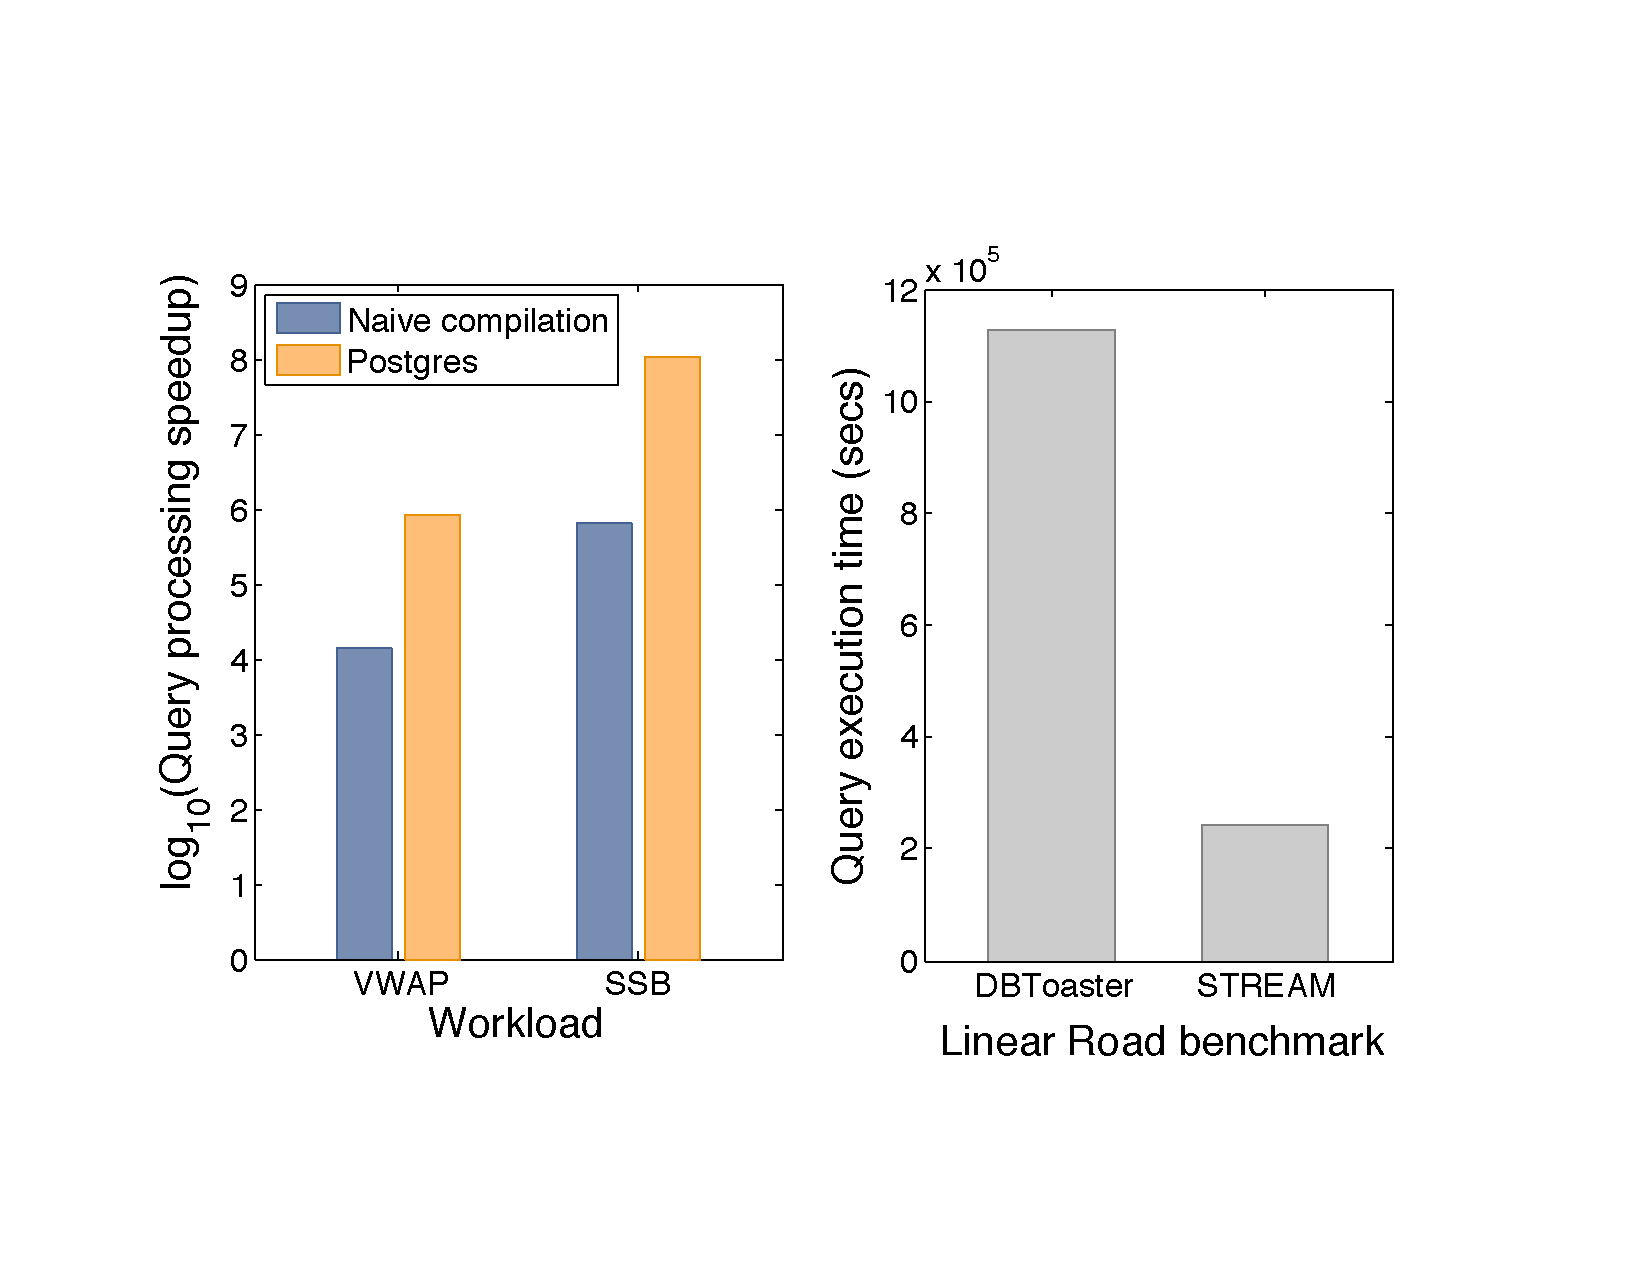
\includegraphics[scale=0.25]{../plots/toaster_comparison}
\end{center}
\caption{Query processing performance comparison of compiled query executors
generated by DBToaster and plan compilation, Postgres and STREAM}
\label{fig:dbtperf}
\end{figure}


\subsection{Adaptive Query Executors}

To this point, we have described a compiler to produce static main-memory query
executor, which incorporates both standard rewrite rules for query optimization
and our custom rules for compilation. The choice of optimal query plans is
subject to the contents of the input relations being processed, leading to the
challenges of query reoptimization and adaptive query processing. In this section
we consider extensions to provide adaptive query execution in our generated code.
For \compiler, this involves producing several plans and generating the
monitoring and decision-making logic to determine which plan to evaluate based on
statistics collected at runtime. We present this section as a discussion of the
relevance and impact of key adaptation techniques in our context, rather than a
focusing on detailed algorithms that reshape such techniques to apply in
\compiler.

\comment{
\subsection{Memory Usage Analysis}
\begin{itemize}
  \item Apply to generalized join graphs, and their hypertree decomposition.
  \item Given a tree-structured join graph, analyse map construction rules and
  discuss based on fanout of nodes in the join graph.
  \item The analysis approach should be to generalize each rewrite rule, compute
  the incremental space usage from each rewrite rule, and finally reason about
  the size of the decomposition tree. The size of this decomposition tree can
  be derived from the hypertree structure.
  \item Consider our standard example template:\linebreak
  $sum(a_1, \ldots , a_n) R,S,T_1,\ldots T_{n-1}$, where there is a $n-way$ join.
  This is a simple join tree of height 2 with $n$ leaves and a single root. Our
  decomposition tree has width $n - level$ at each level and height $n$. The
  number of maps is thus bounded by $\sum_{i=0}^{n-1}{(i+1)*(n-i)} =
  \sum_{i=1}^{n}{(n+1-i)*i} = (n+1)\sum_{i=1}^{n}{i} - \sum_{i=1}^{n}{i^2}$
  \linebreak $= \frac{(n+1)n(n-1)}{2} - \frac{2n^3-3n^2+n}{6} = O(n^3)$.
  Note this includes many duplicate maps, which we'll need to quantify to get a
  tighter bound ($O(n^3)$ is sizeable, even if $n$ is usually small given it's
  the number of relations). Furthermore this does not say anything about the size
  of each map, which we'll have to reason about in terms of the domain sizes for
  each attribute.
  
  \item Assume each leaf in the join tree contributes an aggregation column and
  potentially group-by columns. Internal nodes may or may not contribute
  aggregation columns and group by columns. Internal nodes consist of at least
  one join predicate column.
\end{itemize}
}

\textbf{Batch processing.} 
Simple update or query batching is a common technique used in a variety of query
processors to take advantage of machine-level characteristics in modern computer
architectures, including pipelining, various levels of caches, as well as
vectorized instructions. In addition to these benefits which apply under the hood
of the native code generated, we consider the effects of unrolling the main delta
loop on update batches, creating a table of batch processing functions each
capable of supporting different length batches. While this results in a larger
code size, SQL queries tend to be relatively small and our generated binaries are
on the order of kilobytes or megabytes, and thus code size ifs not a concern at
this stage. We invoke batch processing functions through a signature matching
scheme, where a batch function's signature is simply a specific sequence of data
manipulations (e.g. 4 inserts). For simplicity, and efficient batch detection, we
consider simple patterns as signatures, restricting ourselves to $k$-length
sequences of a single type of data manipulation (i.e. $k$-inserts or $k$-deletes)
for a fixed range of $k$ values.

While more complex batch and pattern detection has been applied, for example for
prefetching as in Scalpel~\cite{bowman-tods:05}, we make the following
observation. As we will see in the experimental evaluation, we produce a highly
efficient executor as the result of our compilation, implying we require a
commensurate improvement in the monitoring conditions that determine when to
adapt running plans. However, these monitoring conditions are typically
implemented by database developers directly in the engine, and are already
operating with low overhead. This entails our design principle that only simple
and extremely lightweight adaptations are of use in a compiled query executor due
to the increasing cost of monitoring relative to processing.

\comment{
\begin{itemize}
  \item Improve pipelining by unrolling the main delta loop, and
  applying independent lines of code in sequence. We refer to applying
  $k$ independent statements in sequence as $k$-level unrolling.
  \item We consider more structured sequences, i.e. patterns perhaps from
  a profiling process based on frequent pattern mining on the delta workload,
  and apply dead-code elimination based on the pattern.
  \item We may want to exploit vectorized instructions, e.g. Altivec/SSE
  instructions. We probably won't go into much depth on this due to limited
  research impact. Generally the goal in this paper is not to build a
  high-performance backend that will take C code and produce tight
  instruction-level code. We leave room for this given our choice of using
  the LLVM framework which will allow modular development of our compilation
  toolchain, but will revisit low-level implementation issues in the future.
  \item Challenge: statically picking the right chunk size for processing, given
  profiling information. We can't handle changes in delta rates to different base
  relations (e.g., no adaptive unrolling/pipelining). How much does this kill the
  argument?
  \item What are the caching effects of bulk operations? Bulk operations should
  improve cache hit ratios as long as the portions of the data structures used
  fit in cache (as working sets). We may want to pick the right chunk size at the
  limit of beneficial pipelining and caching effects, i.e. when one of these two
  advantages starts to become a drawback.
\end{itemize}
}


\textbf{Lazy map maintenance.}
\compiler\ considers evaluating its tuple functions eagerly or lazily, resulting
in a deferred approach to maintaining map structures for producing results given
inputs to other relations. By default, \compiler\ adopts an eager evaluation
strategy, updating map structures for all other parts of the query, given a
single input tuple. Lazy map maintenance is advantageous in scenarios where there
is at least one significantly lagging input, resulting in uncessary eager updates
of the remaining map structures. Taking advantage of the opportunity to be lazy
requires two additional pieces of generated code. The first of these is a simple
profiler that captures update rate statistics to determine candidates for lazy
evaluation. Based on a cost model of these statistics, the second piece of
generated code is a conditional where on one branch, the executor enqueues the
delta to local state associated with the map structure at the point of deferral.
Note we can apply simplifications of those deltas in local state, which may
cancel each other out, or may be merged into a single delta. The tuple function
returns control to the event loop at this point, ready to process the next
available delta.


\comment{  
\textbf{Limitations.}
\begin{itemize}
  \item We profile delta rates on each base relation, and compute internal
  selectivities to determine when to defer updating a map while processing a
  kernel function.
  \item In terms of code generation this adds conditionals based on profiling
  statistics around each map update, where one branch updates the map as before,
  and the other branch stores the delta to be applied at some later point. Note
  given the recursive nature of our decomposition, we jump out of the kernel
  function and handle the next delta on the first branch indicating deferral.
  \item How do we store the deferred updates? As queues associated with each
  map?
  \item This may cause a large number of long jumps in our code, how will this
  affect performance, e.g. what are the effects on branch prediction, I-cache
  performance, etc.?
\end{itemize}
}

\comment{
\subsection{Multi-query compilation and map sharing}
Given that each query is decomposed into a set of map structures, queries
operating on similar sets of input relations are likely to be able to share
such structures in a similar fashion to multi-query optimization. 
}

\comment{
\subsection{Discussion: adaptivity limitations}

\begin{itemize}
  \item Compilation and adaptivity are inherently in tension, pulling engines
  in opposite directions.
  \item TODO: how can we show we are not going to do too badly regardless of how
  the delta workload changes? Perhaps we can borrow ideas from robust query
  processing, where they pick a plan based on maximizing the parameter space
  (i.e. of those statistics profiled) covered by a single plan, as the choice of
  plan we decompose.
\end{itemize}
}


\newcommand{\figurewidth}[0]{1.8in}

\newcommand{\tablefig}[1]{
  \hspace*{-0.25in}
  \includegraphics[width=\figurewidth]{../graphs/graphs/#1}
}

\begin{figure}
\begin{center}
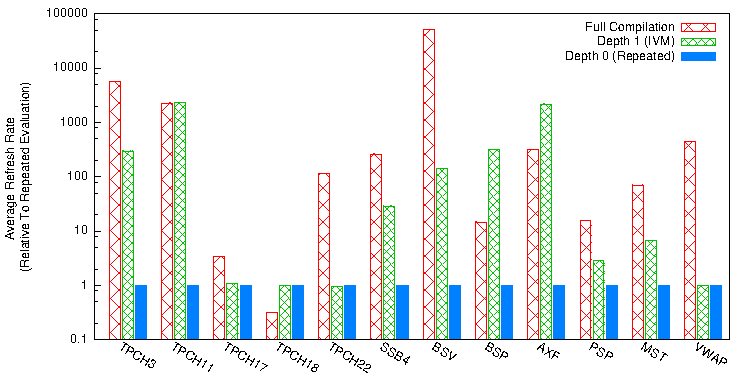
\includegraphics[width=3.4in]{../graphs/graphs/bakeoff.pdf}
\caption{Cross-query comparison of our compiler in different depth-restricted modes, and the best performing streaming and database engine for each query.  Note the logscale on the y-axis.}
\label{fig:experiments:bakeoff}
\end{center}
\end{figure}

\begin{figure*}
\begin{center}

\begin{minipage}{\textwidth}
\begin{center}
\hspace*{0.1in}
\begin{tabular}{cccc}
\tablefig{unified_tpch3.pdf} &
\tablefig{unified_tpch11.pdf} &
\tablefig{unified_tpch17.pdf} &
\tablefig{unified_ssb4.pdf} \\
(a) & (b) & (c) & (d)
\end{tabular}
\caption{TPC-H Query 3~(a), 11~(b), 17~(c), and SSB4~(d): (a) By the 40\%\ marker, all streams except LINEITEM have completed, and the remaining tuples consume no additional memory. (b) For simple two-way joins, full compilation is virtually identical to depth 1. (c) Due to the nested aggregate, IVC requires a nested loop, while full compilation requires only a single scan.(d) Full compilation is a full polynomial order faster than in IVC, although performance does begin to drop once the system begins running out of memory around the 27\%\ marker.}
\label{fig:experiments:tpch3}  
\label{fig:experiments:ssb4}
\label{fig:experiments:tpch17}
\label{fig:experiments:tpch11}
\end{center}
\end{minipage}

\vspace*{0.2in}

\begin{minipage}{\textwidth}
\hspace*{0.1in}
\begin{tabular}{cccc}
\tablefig{unified_brokervariance.pdf} & 
\tablefig{unified_tpch22.pdf} &
\tablefig{unified_vwap.pdf} &
\tablefig{unified_serverload.pdf} \\
(a) & (b) & (c) & (d)
\end{tabular}
\caption{BSV~(a), TPC-H Query 22~(b), VWAP~(c), and SVL~(d):  (a) The many-to-many relationship on the join term forces IVM to perform linear work on each insertion, which full compilation avoids.  (b) The small CUSTOMER stream completes at the 10\%\ marker, while the remaining ORDERS tuples require only linear time with full compilation. (c) IVM repeatedly re-evaluates the nested (parameterized) sub-query, while full compilation maintais a cache of sub-query results. (d) Materializing nested queries gains a polynomial degree of performance over IVM, but memory continues to grow. }
\label{fig:experiments:brokervariance}
\label{fig:experiments:tpch22}
\label{fig:experiments:vwap}
\label{fig:experiments:serverload}
\end{minipage}

\vspace*{0.2in}

\begin{minipage}{\textwidth}
\hspace*{0.1in}
\begin{tabular}{cccc}
\tablefig{unified_pricespread.pdf} &
\tablefig{unified_missedtrades.pdf} &
\tablefig{unified_axfinder.pdf} &
\tablefig{unified_brokerspread.pdf} \\
(a) & (b) & (c) & (d)
\end{tabular}
\caption{PS~(a), MST~(b), AXF~(c) and BSP~(d):  (a,b) The performance and memory plateaus result from a portion of the trace from about 0.001\%\ to 0.01\%, where a single order is repeatedly placed and revoked. (c,d) Full compilation's aggressive materialization strategy results in the caches growing too large to be efficiently maintained.}
\label{fig:experiments:pricespread}
\label{fig:experiments:MST}
\label{fig:experiments:axfinder}
\label{fig:experiments:brokerspread}
\end{minipage}



\end{center}
\end{figure*}

\begin{figure*}
\begin{center}

%\begin{minipage}{\textwidth}
%\begin{center}
%\begin{tabular}{ccc}
%(a) & (b) & (c)
%\end{tabular}
%\caption{TPC-H Query 18~(a). }
%\label{fig:experiments:tpch18}
%\end{center}
%\end{minipage}
%
\vspace*{0.1in}

\begin{minipage}{\textwidth}
\begin{center}
\begin{tabular}{cccc}
\tablefig{unified_tpch18.pdf} &
\tablefig{unified_5gig_tpch3.pdf} &
\tablefig{unified_5gig_tpch11.pdf} &
\tablefig{unified_5gig_tpch22.pdf} \\
(a) & (b) & (c) & (d)
\end{tabular}
\caption{TPCH Query 18 (a): An incorrectly chosen join ordering prevents full compilation from effectively exploiting foreign key dependencies in the TPC-H schema;  The three fastest-running TPC-H queries (3~(b), 11~(c), and 22~(d)) run on a 5GB dataset: (b) Quadratic effects from early parts of the workload become apparent in IVM at this scale, while full compilation remains linear. (c) Maintaining the base relations already projected and aggregated gives a slight edge to full compilation at this scale.  (d) Full compilation performance is reduced due to updates being linear in the size of CUSTOMER, but still performs better than depth 1.}
\label{fig:experiments:big}
\label{fig:experiments:big:tpch3}
\label{fig:experiments:big:tpch11}
\label{fig:experiments:big:tpch22}
\end{center}
\end{minipage}

\end{center}
\end{figure*}

We now analyze the performance of our compilation techniques.  As in Section \ref{sec:dbfail}, our experiments are run on Redhat Enterprise Linux running in a VM with 16 GB of RAM, and 2x4 core Intel Xeon E5620 2.4 GHz processors allocated to it.  Note that our compiler produces single-threaded code, while other platforms were allowed to consume the full resources of the VM.

Our analysis uses the same queries and methodology as in Section~\ref{sec:tscomparison}: The queries are described in Section~\ref{sec:tscomparison:workload}, and expressed in SQL form in Appendix~\ref{app:queries}.

% we analyze our compiler's performance on TPC-H\cite{tpch} Queries 3, 11, 17, 18, and 22, a variant of Star Schema Benchmark\cite{ssb} Query 4 six orderbook queries: VWAP, PS, MST, AXF, BSP, and BSV, and a cluster monitoring query: SVL.  TPC-H queries were modified slightly due to a lack of support for certain advanced features in our SQL parser (e.g., Having, Exists, etc...).  SQL for the queries in our test workload is presented in Appendix

%Our analysis uses the queries from Examples \ref{ex:dbfail:stock} (PS),  \ref{ex:dbfail:tpch} (SSB4), and \ref{ex:dbfail:network} (SVL), Queries numbers 3, 11, 17, 18, and 22 from the TPC-H\cite{tpch} benchmark, the VWAP query presented in \cite{kennedy-ahmad-koch-cidr:11}, and four additional financial queries: MST, AXF, BSP, and BSV in the spirit of VWAP and PS.  The structure of these queries is discussed below.

Queries were run on pre-generated traces until completion of the trace or a 1 hour cutoff was reached.  Traces were generated as follows: The queries: VWAP, MST, AXF, BSP, PS, and BSV were run on a 2.63 million tuple trace of an order book update stream, representing of one day of stock market activity for MSFT.  BID and ASK orders (and cancellations) were translated into equivalent operations on a BIDS and ASKS table, with tuples in either table comprised of a timestamp, an order id, a broker id, a price, and a volume.  The broker id was synthesized for each order -- our experiments use 10 brokers, assigned deterministically based on the order id.  The stream consists of approximately 1.4 million operations on the BIDS table, and 1.14 million operations on the ASKS table.

Queries based on the TPC-H schema (including SSB4) were run on a scaling-factor 0.1 (100 BM) database generated by dbgen\cite{tpch}.  Additional scaling experiments were carried out on TPC-H queries 3 and 11 at scaling factors 0.5, 1, 5, and 10 -- these results are presented in Section~\ref{sec:experiments:bigds}.  Insertions are drawn in-order from each output file of dbgen, with rows from different tables interleaved in random order.  Note that it possible for rows to be inserted before a foreign key constraint has been satisfied, and that smaller datafiles will finish earlier in the stream.  This is not expected behavior in a streaming setting, but provides valuable insights about the performance characteristics of insertions into different tables.

SVL was run on a synthetically generated dataset, simulating 1000 racks of 20 servers each, emitting a total of 100,000 state updates.  The first 20,000 operations in the trace consist of an insertion for each server at 0 load.  For each state update, a random server deletes its previous state tuple and inserts a tuple declaring its new load -- a random real between 0 and 1.

Figure \ref{fig:experiments:bakeoff} compares recursive compilation to the performance of traditional databases and stream processors -- results presented overlap with those of Figure~\ref{fig:queries}.  These numbers speak for themselves, but clearly, traditional engines are not designed for our problem domain.

In order to evaluate our compilation algorithm in a fair environment with a common baseline for performance, we use a depth-limited instantiation of our compilation algorithm: Instead of recursively computing the entire materialization plan, the compiler stops after a fixed number of recursive steps.  Beyond this stage, queries are not materialized and instead computed directly from the base relations.

Compilation at depth-1 is equivalent to traditional IVM techniques, and depth-0 is equivalent to re-evaluating the query on every insertion.  We omit detailed depth-0 performance measurements on graphs where these results are not visible due to scale, or where depth-0 and depth-1 performance are indistinguishable.  Memory measurements are taken using google-perftools\cite{perftools}, and count only memory allocated to the persistent maps and not transient datas (e.g., materialized join results).

As a consequence of the high join width of SSB4, the default materialization plan has an extremely high branching factor (12 at the top level).  Although most materialized views in the plan are duplicates, the compiler must still explore all children of unique nodes -- a prohibitively expensive process.  For the purpose of these experiments, we omit deletions when compiling SSB4 (halving the branching factor).  As SSB4 is a query without nested aggregates, deletions are symmetric with insertions -- In spite of the prohibitive compilation time, the behavior of the compiled query is identical.

\subsection{Equijoins}

We first analyze the performance of our compiler on three equijoin queries with no nested aggregates.  Our compiler recurs only once on TPC-H Query 11.  As a consequence, the result is nearly equivalent to IVM\footnote{We pre-aggregate the materializations of SUPPLIER and PARTSUPP, but this provides only a minor improvement at this scale due to the bounded fanout of this query.}.  

Both TPC-H Query 3 and SSB4 demonstrate a substantial performance increase over IVM.  The one-to-one, and bounded fanout one-to-many relationships between elements of many of these queries are actually advantageous to the IVM implementation -- each insertion only triggers a limited number of reads.  In spite of this, incrementally maintaining the (aggregate) delta queries results in a net reduction in the amount of work required -- especially in a large query like SSB4.

Also note the memory usage of TPC-H Query 3.  Starting by the 40\%\ marker, all streams have been exhausted except for LINEITEM.  The final aggregate's group-by columns are drawn purely from the order table, so insertions into LINEITEM only update aggregate values that have already been allocated by the corresponding ORDER.  Thus, memory usage plateaus for full compilation, while the IVM implementation must continue to store each row.

This is not always true.  For extremely large queries like SSB4 (a 7-way join), the number of intermediate materialized views created is quite large.  Despite the large amount of state that the fully compiled query maintains, any individual update modifies only a small amount of that state, and the fully compiled query's efficiency is unaffected as long as the system has enough memory.  However, memory usage is an important part of the cost/benefit tradeoff of full compilation -- We address a broader range of materialization strategies below in Section~\ref{sec:experiments:othermetrics}.

\subsection{Nested Subqueries}

Figures \ref{fig:experiments:tpch17}c, \ref{fig:experiments:tpch22}b, and \ref{fig:experiments:vwap}c illustrate the performance of our compiler on several queries with nested aggregates.

The lookup over ORDERS in TPC-H Query 22 can be evaluated in constant time both using IVM and full compilation.  However each insertion into ORDERS requires evaluation of the nested aggregate on CUSTOMER, while full compilation maintains a materialized instance of this.

while this value is materialized by the fully compiled version.


queries the CUSTOMER table with two selection conditions: a comparison based on an uncorrelated nested aggregate query over CUSTOMER, and a second based on a lookup (an EXISTS) on ORDERS.   .  

In IVM, insertions into CUSTOMER depend on whether the query optimizer detects that the nested aggregate is uncorrelated and computes it before the rest of the query.  If not, the insertion requires quadratic work, and even if it does, each insertion requires two complete iterations over the customer table: once to compute the aggregate and once to figure out for which customers the state of the comparison changes.  This latter iteration can not be eliminated by full compilation, but the iteration is only over those rows already known to satisfy the selection condition on ORDERS.

VWAP is a query over BIDS with two selection predicates: one over an uncorrelated nested aggregate over BIDS, and one over a correlated (via inequality on the price from the outer BIDS table) nested aggregate over BIDS.  As in TPC-H Query 22, whether the uncorrelated aggregate is an issue for IVM is dependent on the query optimizer.  

The inequality-correlated aggregate is of more interest here.  Because the domain of the correlating variable (price) is determined outside the nested aggregate, the nested subquery must be re-evaluated every time a new price is encountered.  However, the resulting value can then be stored and incrementally maintained.  The domain of prices is bounded, so after an initial ramp up process (that occurs while the size of the table is small) the fully compiled version can incrementally maintain the query output in (close to) constant time.

BSV (Figure \ref{fig:experiments:brokervariance}a) is a two-way aggregate self-equi-join over BIDS.  Despite the lack of a nested aggregate, the performance of BSV follows a pattern similar to the prior two queries.  This is not surprising -- correlated aggregate subqueries are known to be equivalent\todo{cite?} to joining the result with a group-by aggregate query.  Thus, materializing a nested aggregate is tantamount to materializing the first delta.  Furthermore, unlike TPC-H Query 11 (Figure \ref{fig:experiments:tpch11}d), the join relationship is many-to-many, and the benefits of maintaining the join result as an aggregate grow over time.

TPC-H Query 17 is a two-way equi-join over PART and LINEITEM with a correlated nested aggregate over LINEITEM.  Both the join and the correlation are on partkey.  As in the prior queries in this section, incrementally maintaining the nested aggregate makes insertions into PART constant-time rather than linear.  However, even in the fully compiled query, insertions into the LINEITEM table must still iterate over all matching results in the join, which are already being materialized.  

\subsection{5 GB Dataset}
\ref{sec:experiments:bigds}
Figure \ref{fig:experiments:big} presents the behavior of the three fastest TPC-H queries on a scaling factor 5 (5 GB) database.

In the IVM version of TPC-H 3, the one-to-many relationship between them makes each insertion into CUSTOMER linear in the number of LINEITEMS matching CUSTOMER (an average fanout of 40).  A small CUSTOMER table can be processed before many ORDERS are inserted.  With the larger dataset, the increasing cost of insertions into CUSTOMER becomes more pronounced, while the fully compiled version remains constant-time throughout.

Although IVM is nearly identical to full compilation on TPC-H 11, full compilation pushes aggregation into the materialized view while IVM performs the aggregation at lookup.  This, when inserting into SUPPLIER, full compilation reads precisely one value, while IVM reads approximately 80 (and must aggregate over them).  IVM stores both base relations in their entirety, while full compilation stores only the subset needed for query maintenance.  As a consequence, full compilation has a constant, but visible improvement in both performance and memory use at this scale.

Under full compilation, TPC-H Query 22 requires a linear amount of work for insertions into CUSTOMER and a constant amount of work for insertions into ORDERS.  On the small dataset, full compilation was able to get through the CUSTOMER table (note the quadratic behavior in Figure \ref{fig:experiments:tpch22} up to about the 18\% marker) and quickly completed the much larger ORDERS table.  On the larger dataset, full compilation gets bogged down in processing CUSTOMER.

\subsection{Limited Recursion}
\label{sec:experiments:othermetrics}

\begin{figure*}
\begin{center}
\begin{tabular}{|l|c|c|c|c|c|c|}\hline
{\bf Depth} & 1 & 2 & 3 & 4 & 5 & Full \\ \hline 
Avg Rate (refreshes/s) & 5.91 & 0.373 & 0.7 & 12.7 & 51.5 & 50.4 \\ \hline 
Avg Memory per Tuple & 98.5 B & 0.0 B & 0.0 B & 0.0 B & 0.0 B & 61.0 KB \\ \hline 
Lines of Code & 3174 & 12015 & 16517 & 13215 & 10998 & 10431 \\ \hline 
Number of Maps &        6 &       18 &       36 &       45 &       45 &       39 \\ \hline 
\end{tabular}
\caption{Statistics for different compilation depths on SSB4.  Depth-5 is equivalent to full compilation, but also maintains copies of each of the 6 base relations.}
\label{fig:experiments:ssb4depth}
\end{center}
\end{figure*}
We now explore the space of limited recursive compilation beyond IVM.  Figure \ref{fig:experiments:ssb4depth} illustrates the effects of limiting compilation to depths between 0 and 5.  Recall that the maximum recursive depth is one less than the join width of the query.  Thus for SSB4 (which has a join width of 6), compilation to depth-5 is equivalent to full compilation, save that the base relations are maintained and materialized.

At depth-1, the compiled query materializes only the base relations and no intermediate tables.  It must still perform a 5-way join on every insertion, but  only once per update.  The 6 materialized views that it maintains are the 6 base relations from the query.  

At depth-2, the compiled query must now maintain 12 intermediate materialized views, several of which require (effectively) a 4-way join to maintain.  The net cost of maintaining these additional maps does not begin to pay off until depth-4 (where maintenance operations are reduced to at most 2-way joins).  By this point, decomposition has already resulted in the instantiation of all intermediate materializations relevant to the query, so extra and unnecessary work is being done.  

The effectiveness of this approach at depth-4 (in spite of the extra work being done) suggests that a more effective approach to reducing memory consumption might be to materialize not just the set of views closest to the root, but rather a subset of the entire materialization plan (e.g., requiring at most two-way joins throughout the materialization plan).  However, there exists an incredibly large space of possible materialization plans ($2^{39} \approx $ half a trillion possibilities for SSB4) -- cost based optimization within the space of possible materialization plans is future work.

\subsection{Functional Optimizations}
\todo{Yanif}

\subsection{Memory, Extraction, and Future Work}
\label{sec:experiments:future}

\begin{figure}
\begin{center}
\begin{tabular}{|l|c|c|c|}\hline 
\ & Infinite Depth & Depth 1 & Depth 0 \\\hline 
TPCH3 & 2509 & 2855 & 4198 \\\hline
TPCH11 & 531 & 596 & 616 \\\hline
TPCH17 & 928 & 1158 & 1478 \\\hline
TPCH18 & 3668 & 3538 & 4631 \\\hline
TPCH22 & 777 & 1135 & 754 \\\hline
SSB4 & 10995 & 8954 & 7904 \\\hline
BSV & 342 & 327 & 347 \\\hline
BSP & 45625 & 567 & 729 \\\hline
AXF & 2169 & 553 & 1394 \\\hline
PSP & 1442 & 1878 & 1890 \\\hline
MST & 5457 & 2870 & 2434 \\\hline
VWAP & 533 & 466 & 341 \\\hline
\end{tabular}
\caption{Lines of Code Per Query}
\label{fig:experiments:loc}
\end{center}
\end{figure}

It is important to understand not only where our compiler succeeds, but where its limitations lie.  We now consider several cases where the observed performance of our technique does not match up with our (high, and perhaps naive) expectations.  As a consequence of our experimentation and analysis, we have identified three core challenges for future work in this area.

\tinysection{Join Ordering}
The first case of poor performance we consider is TPC-H Query 18 (Figure \ref{fig:experiments:tpch18}a), a three-way join over CUSTOMER, ORDERS, and LINEITEM, with an EXISTS predicate over a query that itself has a nested aggregate as a condition.  Although the query effectively involves two levels of nesting, it is otherwise quite simple.

Yet in spite of the simplicity, the query performs badly -- the query performs better at depths 0 and 1.  The reason for this poor performance is our join ordering heuristic: The trigger that updates the query result must compute a join between the delta of the extracted nested subquery (aggregated over orderkey) and a materialized representation of CUSTOMER $\bowtie$ ORDER $\bowtie$ LINEITEM (aggregated over custkey and orderkey).  

Not knowing about the one-to-many relationship between custkey and orderkey, we iterate over the materialized join first and effectively iterate over all orders placed so far.  Join ordering is a well studied problem in the database community, and the solution to this problem is purely an engineering challenge.  A further unfortunate side effect of the incorrect join ordering is that the added (unnecessary) looping involves lookups that extend the domain of several intermediate materialized views, causing an explosion of memory use.

\tinysection{Domain Maintenance}
The second case is best illustrated by SVL (Figure \ref{fig:experiments:serverload}d), a query over a single SERVERS table with a single selection predicate based on two uncorrelated aggregates.  By all rights, this query should perform as well as TPC-H Query 22, VWAP, and BSV (Figure \ref{fig:experiments:tpch22}).  The difficulty here is related to domain maintenance \todo{Do we discuss this elsewhere in the paper?  Backreference... this is not the place to be discussing it}.  In effect, our runtime is unable to properly garbage collect deleted entries in one of the materialized views, resulting in a progressively growing workload on every insertion.  

A similar issue affects both PS and MST (Figures \ref{fig:experiments:pricespread}a, and \ref{fig:experiments:missedtrades}b respectively), both two-way joins over BIDS and ASKS.  In both queries there are two selection predictaes: one comparing a column of ASKS to nested subquery over ASKS, and a similar predicate over BIDS.  Apart from a stretch of updates (0.001\%\ to 0.01\%\ in the trace) in the stock market trace where the same order is repeatedly placed and revoked the query performance follows a very similar performance curve. 

\tinysection{Map Extraction}
The final case of performance issues is seen in both AXF (Figure \ref{fig:experiments:axfinder}c) and BSP (Figure \ref{fig:experiments:brokerspread}d), both simple two-way inequality joins.  Our aggressive extraction heuristic attempts to materialize the entire delta query, which for inequality joins includes an unbound variable.  In such cases, the extracted expression is incrementally maintained for every encountered valuation of the unbound variable.  Thus, each change to the extracted expression requires an iteration over all previously encountered values.  In most cases, most of the state kept for each row in this output can be pre-aggregated and is typically quite small.  However, in the case of these two queries, these tables are each approximately the size of both input tables.  An improved, data-dependent extraction heuristic could identify such situations and compute the inequality join inline -- effectively doing what IVM does.  Alternatively, the entire materialized delta could be incrementally maintained more efficiently using datastructures suited to computing aggregates over ranges (e.g., \cite{range trees}).

\tinysection{Summary}
Our compilation technique is effective on select-project-join-aggregate queries involving equi-joins and nested subqueries which are uncorrelated, correlated through an equality comparison, or correlated on a variable (or variables) with a small domain.  It is especially good on queries with small result sets (but large inputs).

Our technique is less effective on inequality joins and nested aggregates correlated through an inequality -- although both are still handled efficiently if the domain of the values being compared is small.  In a similar vein, we do not optimize to take advantage of, or avoid problems caused by data-specific characteristics (e.g., foreign keys, large domains, etc\ldots). 



\begin{figure}
\begin{center}
\end{center}
\end{figure}




\section{Related Work}

To the best of our knowledge, there has been limited research literature
addressing the question of how to compile continuously evaluated SQL queries to
a low-level imperative language such as C++.  With this in mind, in this section
we contrast our map calculus, compilation algorithm and generated engine to
several more extensively investigated topics, namely view maintenance,
main-memory databases as well as stream and event processing.

\textbf{Database compilers and generators.}
Database management systems have long realised the benefits of compilation in
their ability to \textit{prepare} and execute SQL queries and stored procedures
since the days of System R~\cite{chamberlin-tods:01}, which investigated
compilation to machine code for computing architectures from that era. To the
best of our knowledge, modern database systems do not generate assembly, rather
compilation produces query plans -- a network of operators implementing the
relational algebra, and fundamentally processing with a Volcano-style
iterator-based approach~\cite{graefe-tkde:94}. We view query plans as
interpreted programs, that is while the operators themselves have efficient
implementations, the plan is a data structure representing a composition of
operators, and must be inspected, and dispatched by the query execution engine
(i.e the interpreter). 
Furthermore, in such systems, continuous query processing
is often an afterthought, and added in the form of triggers, views and
incremental view maintenance algorithms. In contrast our approach to compilation
generates engines that differ significantly from plan-based approaches in that
our generated code is designed for per-tuple processing, and thus streaming, and
does not incur any of the overhead of having to inspect plan data structures.

Other related works have looked at the issue of database generation, for example
the work by Batory et al. on the GENESIS~\cite{batory-tse:88} system. Such work
is much more in the spirit of extensible database systems, such as Starburst and
Postgres. We focus purely on the query processing aspect, in the main-memory
context, as opposed to attempting to define database generation languages, or
tools to support modular database architectures.


\textbf{View maintenance.}
View maintenance algorithms are in abundance in the database literature, with
topics ranging from efficient view maintenance algorithms given base relation
deltas~\cite{colby-sigmod:96}, which may be eagerly or lazily
applied~\cite{yan-vldb:95,zhou-vldb:07}, to the question of which views to
actually materialize and how to use such views during query
optimization~\cite{kotidis-tods:01,zhou-icde:07}.
Zhou et al.~\cite{zhou-vldb:07} describe a lazy view materialization technique,
where their computation of deltas from single tuples starts from a similar point
to ours, however, their approach does not generalize like our map calculus,
particularly in the case of nested aggregations such as the VWAP query seen in
this work.
Griffin and Libkin~\cite{griffin-sigmod:95} study the problem of incremental
view maintenance for relations with duplicates, using a bag algebra to derive
update rules.  
More pertinent to the main-memory database context,
Roussopoulos~\cite{roussopoulos-tods:91} presents a pointer-based approach to
implement views with ViewCache.
Our map calculus differs in that it inherently computes a set of maps to support
incremental maintenance of a query result, rather than a single view. None of
these works consider any form of multi-level view maintenance attained via
recursive compilation.
\comment{
Our approach to selecting maps under a memory constraint differs from
traditional cost models to choose views to materialize, given our top-down approach to
decomposing queries with maps.
Furthermore, given our target application of non-interactive queries and a static
query workload, we need not maintain base relations, unlike standard relational
query processors which do so to provide ad-hoc query capability at the expense of
orders of magnitude performance as seen in our experimental section. This
obviates the need for any pointer or index-based approach to track back to
original base relation tuples, unlike existing main-memory database systems. Most
critically, the notion of compiling these view maintenance algorithms is clearly
a simple and effective technique for generating query executors for unmatched
performance.
}
\comment{
\begin{itemize}
  \item Asymmetric increment techniques \cite{yang-icde:05}.
  \item Group-by optimizations \cite{yan-icde:94}.
\end{itemize}
\noindent \textbf{DataCubes}
\begin{itemize}
  \item Classical literature \cite{gray-icde:96,mumick-sigmod:97}.
  \item TODO: more papers if we head into cubes.
\end{itemize}
}

\noindent \textbf{Stream and event processing.}
Our work can loosely be compared to complex event and stream processing
engines~\cite{wu-sigmod:06,agrawal-sigmod:08,white-pods:07,motwani-cidr:03,abadi-vldbj:03}
due to the common goal of handling frequently changing data.
SASE+~\cite{agrawal-sigmod:08} and Cayuga~\cite{white-pods:07} are complex event
processors that focus on sequence and pattern query processing on event streams
using NFA-based approaches to process a variety of patterns including Kleene
closures and negation operators. Relational stream processing engines such as
STREAM~\cite{motwani-cidr:03} and Aurora~\cite{abadi-vldbj:03} investigate
continuous query processing architectures that are capable of evaluating
stream-equivalent versions of the standard relation algebra.
\comment{From the systems
perspective, several novel techniques were developed including scheduling, load
shedding, and approximate query processing.
}
Many of these systems are simultaneously addressing the issue of efficiency and
the semantic requirements of their target applications, exploiting such semantic
properties to attain performance. In contrast, our approach does not use such
novel data and query models -- we focus on standard relational queries, but
critically address performance issues of arbitrary updates to a database snapshot. We
also argue for an alternative to plan-based execution, and design query
executors to best suit continuous execution in a main-memory environment.

We briefly comment on two other recent works on data stream processing. first
the SPADE~\cite{gedik-sigmod:08} language designed for IBM's System S stream
processing engine. SPADE is a declarative language for specifying data stream
applications, however the authors do also discuss their implementation including
their compilation process. The authors discuss compiler optimizations such as
operator grouping for execution across multiple hardware contexts, and operator
fusion to reduce internal queueing. Note that \compiler\ completely eliminates
any internal queueing, since we produce a single-straight line function, and
automatically derives appropriate data structures to support query processing
via a single function. This latter issue is not considered in SPADE. Finally,
StreamBase~\cite{streambase}, a commercialization of the Aurora stream
processing engine has also studied the problem of compiling stream programs,
however there is little documentation~\cite{sb-patent} regarding the technical
details of their techniques. To the best of our knowledge, their compilation
process does not include generating straight-line processing functions in the
same aggressive manner as \compiler.

 \comment{
 TODO:
contrast our work to the above -- we avoid the need for windows or punctuations
by making adopting an insert/delete/update stream model, and assuming that the
base relations always fit in memory (i.e. \#deletes/updates is proportional to
\#inserts). Stream processors still evaluate an operator-centric query plan,
hence they cannot exploit compiler optimizations on a query processing kernel
function. They also do not deal with maintaining precomputed partial results as
we do with our map decompositions. What can we say about complex event processors
and the NFAs they evaluate?


\begin{itemize}
  \item STRIP: rule-based maintenance of derived data, with finance app example \cite{adelberg-sigmod:97}
\end{itemize}
}

\comment{
\noindent \textbf{Compiling high-level languages for embedded systems.}
The embedded systems community has partially studied on compiling high-level
languages into a low-level imperative target language.
Newton et al.~\cite{newton-lctes:08} present WaveScript, a scripting language
for processing windows, or segments, of a data stream, and describe a compiler to
construct stream dataflow graphs that are capable of running on XScale CPUs.
WaveScript programs are transformed into dataflow graphs, which may in turn be
manipulated by algebraic rewrite rules, similar to a query optimizer. However,
WaveScope does not address relational queries.
Toman and Weddell~\cite{toman-dbtel:01} describe the DEMO system which compiles
SQL queries into Java or C code, implementing query plans as navigational plans
that utilize pointer access in place of scans and indexing, and supporting query
functionality over existing data structures for an embedded program. The authors
use integrity constraints in their compiler to describe the relationship between
schemas and the physical data structures used by an embedded program, and in turn
generate navigational plans and iterators, which can be used to produce C code in
a straightforward manner. DEMO has taken a theoretical approach to describe
their compilation, and does not consider systems issues nor have they released
a prototype and provided an effective tool to perform compilation.
}


\noindent \textbf{Main memory databases.}
Early work on main-memory databases studied how to reduce the bottleneck effect
of a variety of I/O tasks including recovery tasks such as checkpointing, as well
as logging and locking structures \cite{bohannon-sigmod:99}. There have been
several recent efforts on this topic given the developments in main memory,
including MonetDB/X100~\cite{boncz-cidr:05}, H-Store~\cite{kallman-pvldb:08},
and Blink~\cite{raman-icde:08}.
\comment{
Boncz et al.~\cite{boncz-cidr:05} present the MonetDB/X100 database engine, a
high-performance column-oriented database, that leverages techniques such as
vectorized processing and loop pipelining on chunks of columns while evaluating
operators in query plans. Kallman et al.~\cite{kallman-pvldb:08} describe
H-Store, a shared-nothing distributed main memory database to provide high
throughput processing on OLTP workloads. H-Store achieves its performance through
careful deployment of horizontally partitioning of relations, and localizing OLTP
transactions to partitions. Raman et al.~\cite{raman-icde:08} describe Blink, a
row-oriented main memory query processor that extensively uses compression on
denormalized relations, and applies aggregates while scanning these relations as
its main query processing functionality.
}

These interest in these systems highlight the potential for exploring
main-memory database architectures, but derive from standard plan-based query
processing techniques, and do not study compilation.  For now we have looked at
describing queries as tuple functions, and exploit aggressive recursive
compilation. Having only started generating our runtime, we can now
proceed to the systems level aspects of our tuple functions, for example
investigating cache performance in much greater depth, and in particular
understanding which of the above techniques and optimizations can be applied in
our context, as well as leveraging relevant work from the compiler and
programming languages communities.

\section{Conclusions and Future Work}

We have presented \compiler, a SQL compiler that comprehensively shows the
benefits of creating compiled query executors for main-memory procesing of
repetitive and standing queries. Our executor is based on the notion of
processing individual tuples, by combining them with aggregated views defined
over the remaining parts of the query. The tuple function is also responsible for
maintaining these aggregate views, and this turns out to be extremely simple and
cheap in the main memory context given our novel map algebra which can readily
convert single tuple deltas into simple arithmetic expressions of parameterized
queries. Our implementation of \compiler\ dominates state of the art database
systems, including relational databases and stream processing on a variety of
application scenarios, and is only rivalled in a small set of use cases by a
compiled query executor implementing a plan in its original operator-centric
form. In our view, this raises the possibility that such an approach should be
the de facto processing methodology, as opposed to the plan-based approach in
future query executors.

We view the topic of query compilation and compiled executors as still in its
infancy, and hope that \compiler\ is able to raise interest in this domain. 
As part of ongoing and future work, we plan to investigate the efficiency of
our generated code and understand its memory behavior. A large part of this
includes extending to other non-relational operations in SQL, such as top-k,
and understanding the data structures needed to process tuple functions for
such operations. Furthermore, we would like to apply tuple function
compilation and execution in other novel domains where the database
community is branching out, including scientific databases for executing
simulations, as well as for probabilistic inference on graphical models, where
the common theme in both these domains is a graphical representation of 
computation. Finally the question of getting the right balance of adaptivity
and compilation, especially in light of the difficulty in managing large-scale
datbaase systems, remains an open question. We would like to integrate our
compilation techniques with the emerging techniques for providing self-managing
databases to address this issue,

\comment{
\begin{itemize}
\item
Programming language theory paper: how to compile SQL to use user-specified
data structures.

\item
Compiling down more general declarative languages, with operators and
aggregates whose semantics is definable in the framework. Applications e.g.\
probabilistic inference in graphical models. Compile the graph structure
of the graphical model and the inference algorithms (using e.g.\ mesage
passing techniques) into C code. The data to be processed are the factor
relations/conditional probability tables.

\item
Compiling database applications and the database server together into a single
program that runs robustly and requires no administration. I.e., combine
our query compilation work with automatic administration ideas, if any of
this is actually needed.
\end{itemize}
}


%\footnotesize{
\small{
\bibliographystyle{abbrv}
\bibliography{ref}
}

\end{document}
